\documentclass{ctexart}
\usepackage{lipsum}
\usepackage{graphicx}
\usepackage{cite}
\usepackage{afterpage}

\usepackage[section]{placeins}
\newcommand\blankpage{%
    \null
    \thispagestyle{empty}%
    \addtocounter{page}{-1}%
    \newpage}
\usepackage{mystyle}
\usepackage{longtable}
\usepackage{siunitx}
\begin{document}

\section{拟合RAA分母参数} % (fold)
\label{sec:拟合raa分母参数}

用Levy函数猜测\textbf{分母}pp碰撞中B粒子$p_T$分布,并带入\texttt{PYTHIA8}中产生B0$\to$e的事例,与实验数据b$\to$e\cite{Aidala:2019hib}对比。\par
1.首先检查\texttt{PYTHIA8},FONLL与实验数据符合情况。第二行使用FONLL的B分布$\rd N/\rd p_T$,带入程序中调用PYTHIA8,得到B0$\to$ e的$\rd^2N/2\pi p_T\rd p_T\rd y$(${\abs{y}<0.7}$). 第三行使用FONLL直接计算b$\to$e 的子粒子$\rd^2N/2\pi p_T\rd p_T\rd y$,第4行是相对误差。
\begin{longtable}{l|lll}\hline
$pT$ & fonll B 数据+PYTHIA8 B$\to$e & fonll e数据  & 相对误差                  \\\hline
1.1  & 4.39E-06                  & 4.5138E-06 & -0.028485976339227    \\
1.2  & 3.94E-06                  & 4.0204E-06 & -0.019560988956323    \\
1.3  & 3.50E-06                  & 3.5573E-06 & -0.014982430495038    \\
1.4  & 3.08E-06                  & 3.1207E-06 & -0.013734739000865    \\
1.5  & 2.70E-06                  & 2.7109E-06 & -0.003983068353683    \\
1.6  & 2.35E-06                  & 2.3455E-06 & -1.24493711360564E-05 \\
1.7  & 2.02E-06                  & 2.0196E-06 & 0.000619875222816     \\
1.8  & 1.74E-06                  & 1.728E-06  & 0.006375347222222     \\
1.9  & 1.49E-06                  & 1.4736E-06 & 0.012432206840391     \\
2    & 1.27E-06                  & 1.2538E-06 & 0.015408358589887     \\
2.1  & 1.08E-06                  & 1.0645E-06 & 0.01645016439643      \\
2.2  & 9.20E-07                  & 9.0241E-07 & 0.019024944315777     \\
2.3  & 7.78E-07                  & 7.6381E-07 & 0.018595462222281     \\
2.4  & 6.57E-07                  & 6.4636E-07 & 0.016364874063989     \\
2.5  & 5.59E-07                  & 5.4668E-07 & 0.021683617472745     \\
2.6  & 4.73E-07                  & 4.6245E-07 & 0.02192020759001      \\
2.7  & 4.02E-07                  & 3.913E-07  & 0.026131101456683     \\
2.8  & 3.39E-07                  & 3.316E-07  & 0.023472255729795     \\
2.9  & 2.89E-07                  & 2.8109E-07 & 0.028584190117044     \\
3    & 2.45E-07                  & 2.3841E-07 & 0.027183842959607     \\
3.1  & 2.09E-07                  & 2.0236E-07 & 0.032720794623443     \\
3.2  & 1.77E-07                  & 1.7196E-07 & 0.028005931612003     \\
3.3  & 1.50E-07                  & 1.4629E-07 & 0.025248000546859     \\
3.4  & 1.28E-07                  & 1.2461E-07 & 0.028309525720247     \\
3.5  & 1.09E-07                  & 1.0635E-07 & 0.024464598025388     \\
3.6  & 9.36E-08                  & 9.0946E-08 & 0.029607349416137     \\
3.7  & 7.99E-08                  & 7.7959E-08 & 0.024703626265088     \\
3.8  & 6.89E-08                  & 6.6817E-08 & 0.030445245970337     \\
3.9  & 5.92E-08                  & 5.7387E-08 & 0.032295990381097     \\
4    & 5.08E-08                  & 4.9366E-08 & 0.029825993598833     \\
4.1  & 4.36E-08                  & 4.2553E-08 & 0.023774586985642     \\
4.2  & 3.75E-08                  & 3.6748E-08 & 0.021501306193534     \\
4.3  & 3.25E-08                  & 3.1777E-08 & 0.024101079397048     \\
4.4  & 2.83E-08                  & 2.7539E-08 & 0.02918628127383      \\
4.5  & 2.46E-08                  & 2.3908E-08 & 0.027296595281914     \\
4.6  & 2.13E-08                  & 2.0794E-08 & 0.022078243724151     \\
4.7  & 1.86E-08                  & 1.8112E-08 & 0.026525894434629     \\
4.8  & 1.61E-08                  & 1.581E-08  & 0.020662049335863     \\
4.9  & 1.42E-08                  & 1.3823E-08 & 0.026796064530131     \\
5    & 1.22E-08                  & 1.2105E-08 & 0.008560346964064     \\
5.1  & 1.08E-08                  & 1.0615E-08 & 0.015965049458314     \\
5.2  & 9.56E-09                  & 9.3195E-09 & 0.026167712860132     \\
5.3  & 8.40E-09                  & 8.1919E-09 & 0.024804013720871     \\
5.4  & 7.33E-09                  & 7.2119E-09 & 0.016800704391353     \\
5.5  & 6.48E-09                  & 6.3629E-09 & 0.018919832152006     \\
5.6  & 5.64E-09                  & 5.6212E-09 & 0.003585711236035     \\
5.7  & 5.03E-09                  & 4.9735E-09 & 0.012288730270433     \\
5.8  & 4.46E-09                  & 4.4064E-09 & 0.012119417211329     \\
5.9  & 3.96E-09                  & 3.9097E-09 & 0.012963654500345     \\
6    & 3.52E-09                  & 3.4734E-09 & 0.0125367075488       \\
6.1  & 3.12E-09                  & 3.0888E-09 & 0.010738150738151     \\
6.2  & 2.79E-09                  & 2.7515E-09 & 0.012843830637834     \\
6.3  & 2.47E-09                  & 2.4542E-09 & 0.006704751039035     \\
6.4  & 2.20E-09                  & 2.1918E-09 & 0.002897207774432     \\
6.5  & 1.96E-09                  & 1.9595E-09 & -0.000152589946415    \\
6.6  & 1.76E-09                  & 1.7542E-09 & 0.002255843119371     \\
6.7  & 1.57E-09                  & 1.5716E-09 & -0.003120005090354    \\
6.8  & 1.40E-09                  & 1.4098E-09 & -0.009870194353809    \\
6.9  & 1.27E-09                  & 1.2662E-09 & -5.53625019744211E-05 \\
7    & 1.13E-09                  & 1.138E-09  & -0.004093321616872    \\
7.1  & 1.01E-09                  & 1.0242E-09 & -0.017198594024605    \\
7.2  & 9.10E-10                  & 9.2255E-10 & -0.013241450327896    \\
7.3  & 8.20E-10                  & 8.3194E-10 & -0.014462821838113    \\
7.4  & 7.40E-10                  & 7.5106E-10 & -0.014287540276409    \\
7.5  & 6.58E-10                  & 6.7824E-10 & -0.029669143665959    \\
7.6  & 6.04E-10                  & 6.1347E-10 & -0.015800283632451    \\
7.7  & 5.46E-10                  & 5.5507E-10 & -0.016733204821013    \\
7.8  & 4.93E-10                  & 5.0272E-10 & -0.019638765117759    \\
7.9  & 4.45E-10                  & 4.5574E-10 & -0.023932285952517    \\
8    & 4.01E-10                  & 4.1379E-10 & -0.032068440513304    \\
8.1  & 3.63E-10                  & 3.7553E-10 & -0.034631587356536    \\
8.2  & 3.29E-10                  & 3.4164E-10 & -0.035534773445732    \\
8.3  & 2.99E-10                  & 3.1059E-10 & -0.036285424514633    \\
8.4  & 2.70E-10                  & 2.827E-10  & -0.045855146798727    \\
8.5  & 2.44E-10                  & 2.5757E-10 & -0.051947820010095    \\   \hline
\end{longtable}
进一步,将FONLL数据与实验数据\cite{Aidala:2019hib}对比知,FONLL误差较大。
\begin{tabular}{llll}\hline
pT   & 实验数据     & FONLL数据  & 误差                 \\\hline
1.1  & 1.05E-05 & 4.39E-06 & -0.58236           \\
1.3  & 7.34E-06 & 3.50E-06 & -0.522615395095368 \\
1.5  & 5.22E-06 & 2.70E-06 & -0.482739022988506 \\
1.7  & 3.72E-06 & 2.02E-06 & -0.456760241935484 \\
1.9  & 2.65E-06 & 1.49E-06 & -0.437011283018868 \\
2.1  & 1.90E-06 & 1.08E-06 & -0.430520421052632 \\
2.3  & 1.35E-06 & 7.78E-07 & -0.423693777777778 \\
2.5  & 9.69E-07 & 5.59E-07 & -0.423597523219814 \\
2.7  & 6.95E-07 & 4.02E-07 & -0.422266043165468 \\
2.9  & 5.01E-07 & 2.89E-07 & -0.422904730538922 \\
3.1  & 3.62E-07 & 2.09E-07 & -0.422703370165746 \\
3.3  & 2.63E-07 & 1.50E-07 & -0.429720418250951 \\
3.5  & 1.92E-07 & 1.09E-07 & -0.43254265625     \\
3.7  & 1.40E-07 & 7.99E-08 & -0.429393785714286 \\
3.9  & 1.03E-07 & 5.92E-08 & -0.424850776699029 \\
4.25 & 6.20E-08 &          &                    \\
4.75 & 2.99E-08 &          &                    \\
5.5  & 1.11E-08 & 6.48E-09 & -0.41592027027027  \\
6.5  & 3.04E-09 & 1.96E-09 & -0.355525986842105 \\
7.5  & 9.20E-10 & 6.58E-10 & -0.284655217391304 \\
8.5  & 3.03E-10 & 2.44E-10 & -0.194093069306931 \\\hline          
\end{tabular}



\par
2.定义误差$\displaystyle x=\pare{\frac{o-e}{e}}^2 $\footnote{实际上应该使用统计量$\displaystyle\chi^2=\+/(o-e)^2/e/$,使用$x$是事前未发现,只是需要让相对误差平方和最小。}。其中$o$是MonteCarlo算出来的,e是实验数据。 使用模拟退火法,得到Levy函数三个参数值, 如图\ref{b2e}所示。\footnote{$\square{}$是由于ROOT出现问题无法显示,实际上是$-$}
\[p_1 = \num{3.61558e-05}\quad p_2 = \num{0.669567}\quad p_3 = \num{9.740049}\quad x=\num{1.30434e-01} \]
\begin{figure}[h]\centering
	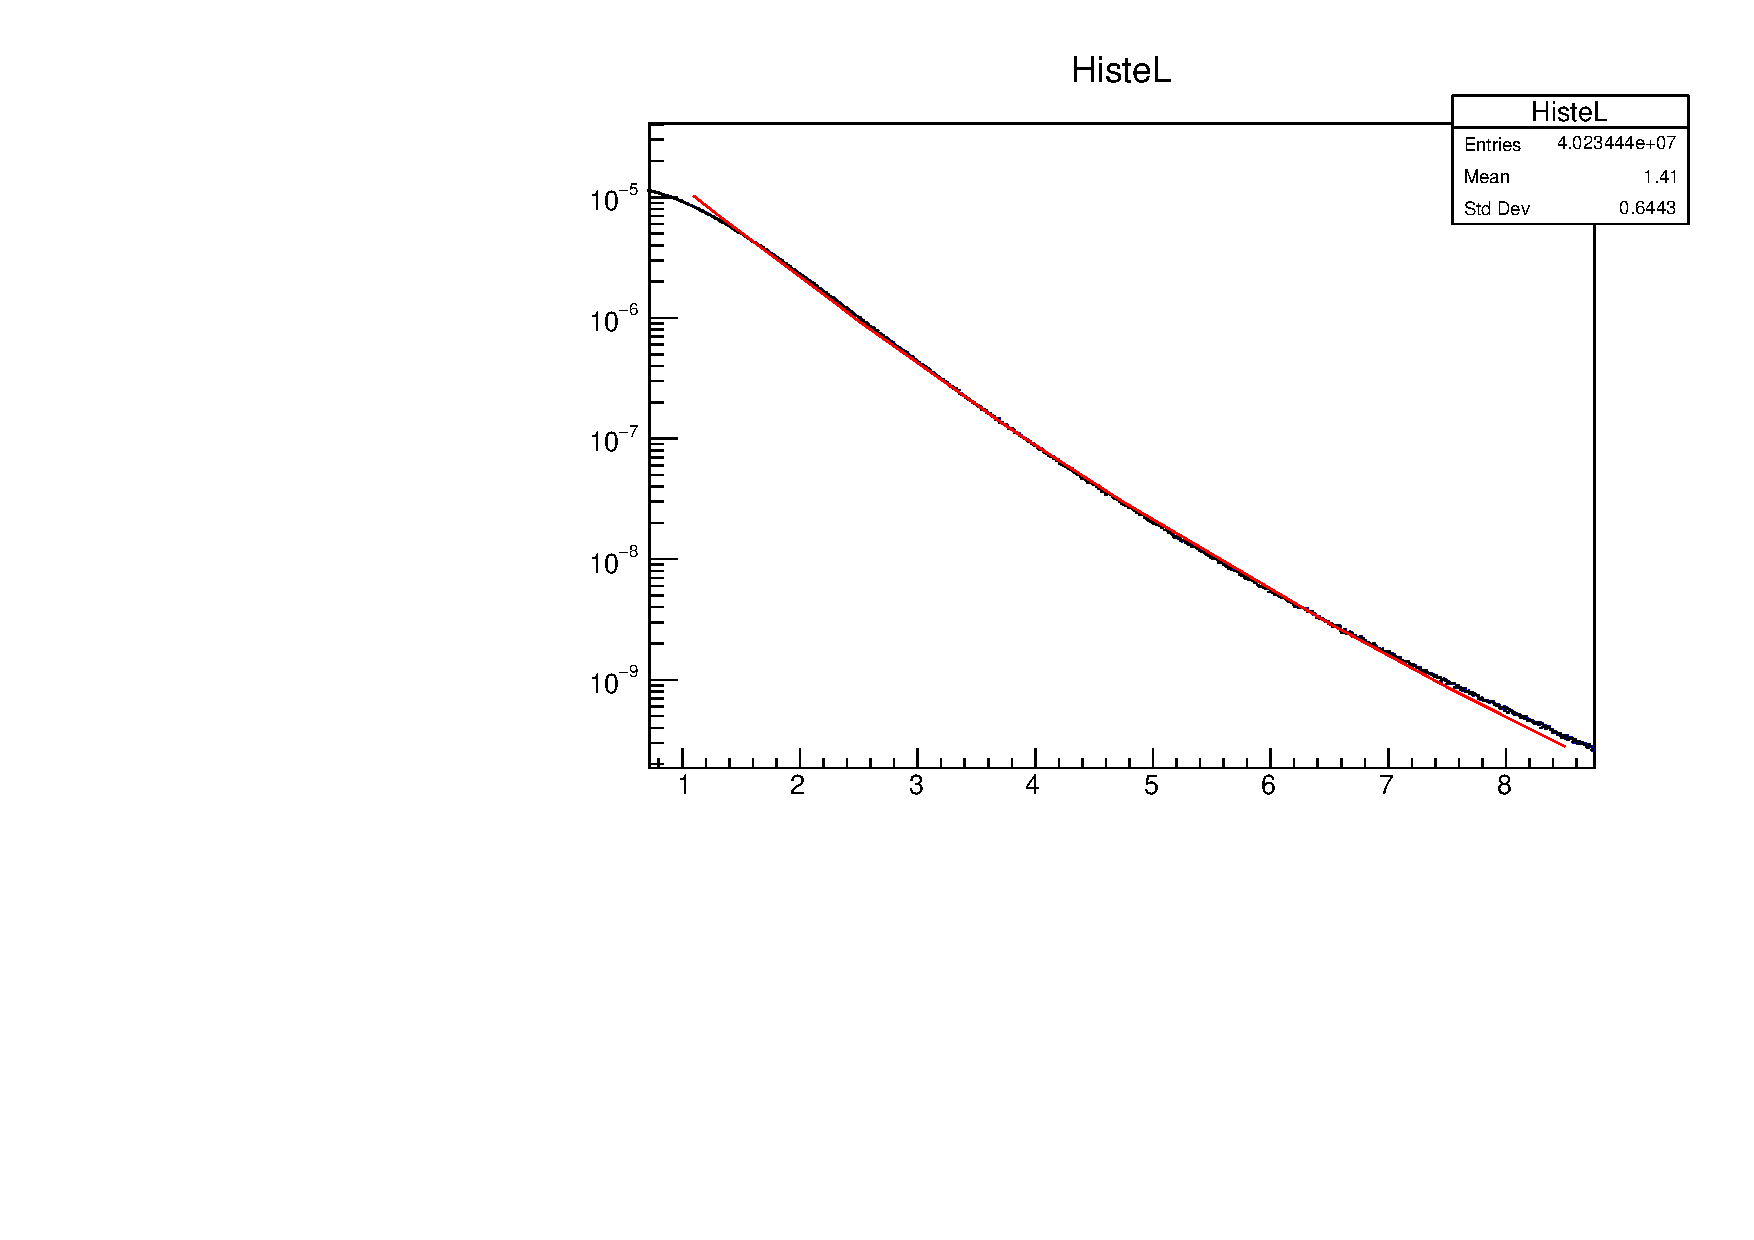
\includegraphics[width=8cm]{src/b2elog.pdf}
	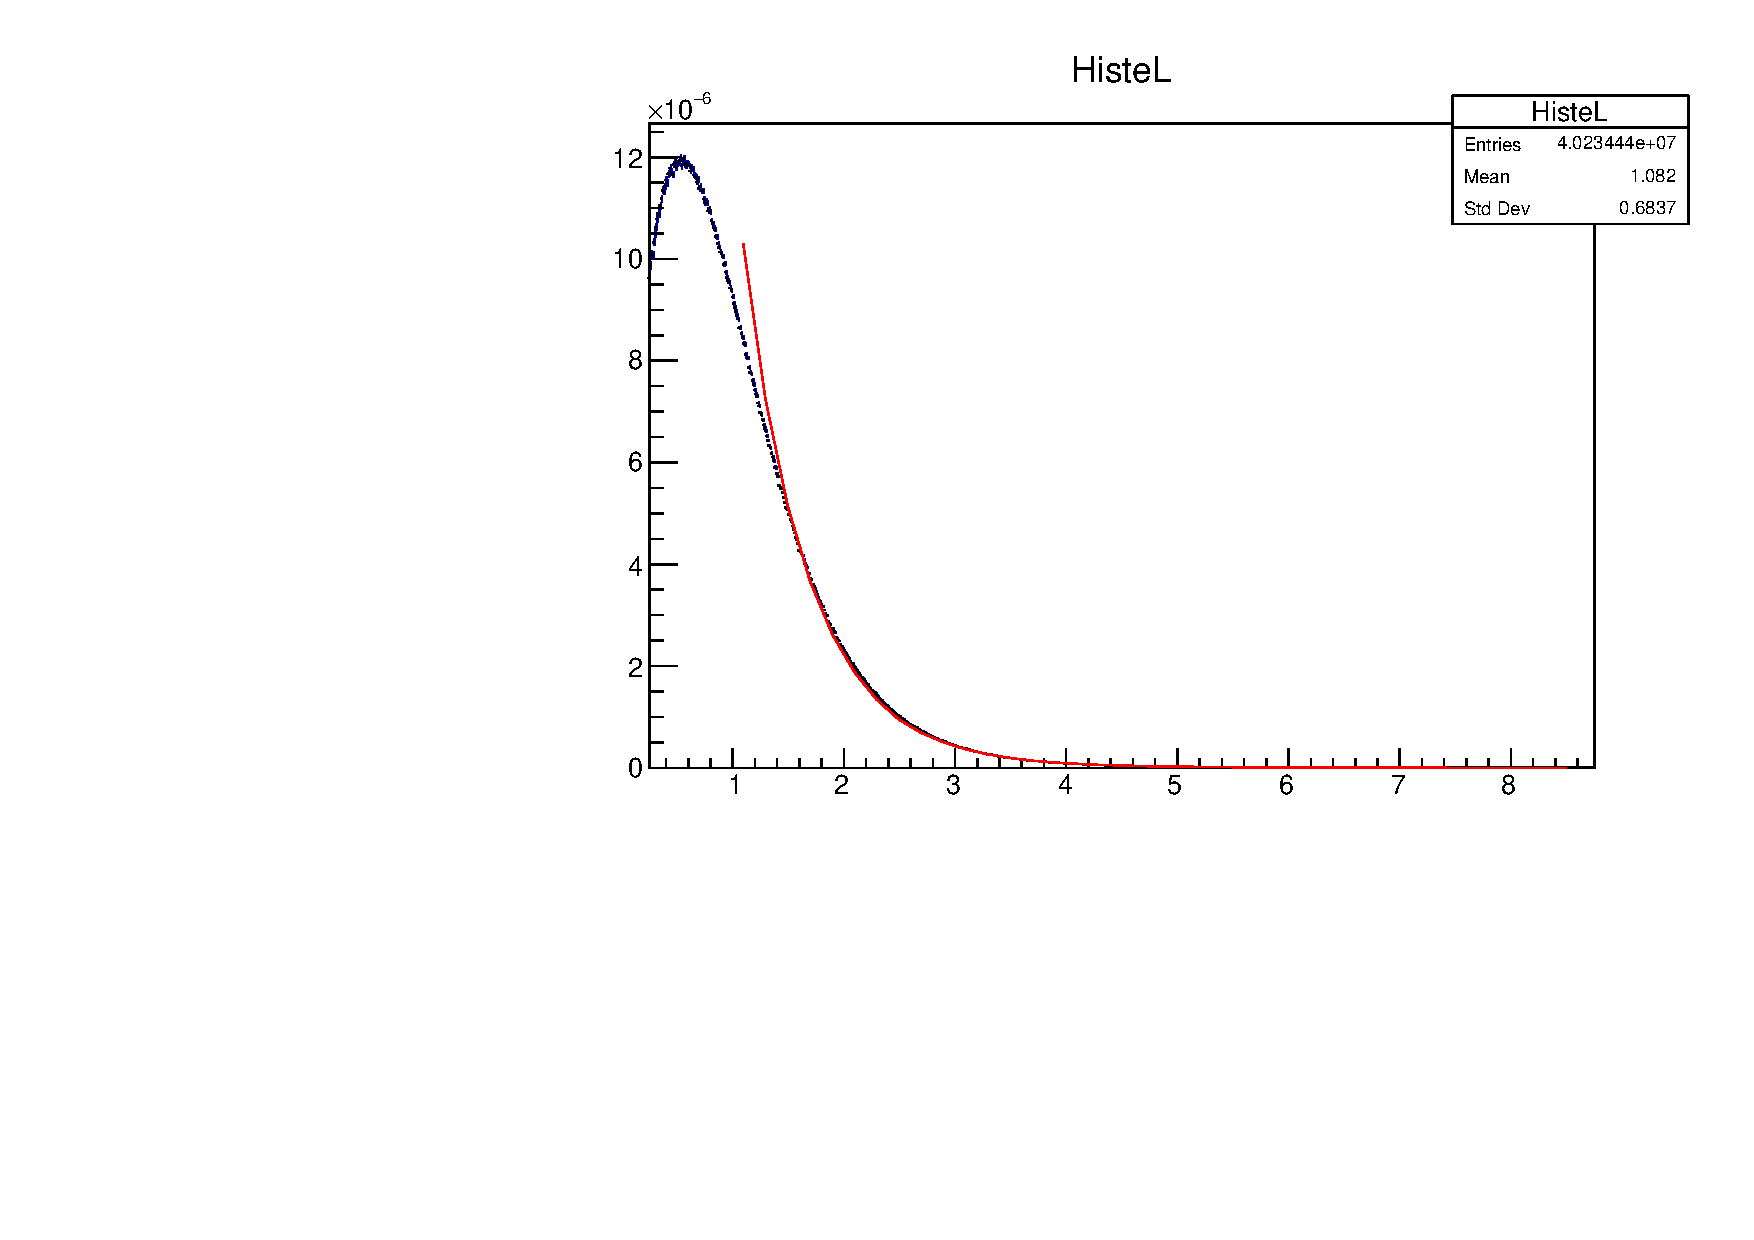
\includegraphics[width=8cm]{src/b2e.pdf}
	\caption{B0$\to$e实验测出的结果(红线)和模拟结果(蓝线)的比较, 纵坐标是$\rd\sigma/2\pi p_T\rd p_T\rd y$ }
	\label{b2e}
\end{figure}
Levy函数有三个参数,设为$\+vp=(p_1,p_2,p_3)$。
模拟退火法算法为(假设上一步输出的参数$\+vp‘$, $x’$已经算出)
\begin{enumerate}
	\item 初始化,设定步长$\+v\epsilon$,设定温度与步数的函数$T=0.95^{-i}$,$i$是步数。
	\item 产生一个分布在$[-1,1]^3$的随机向量$\+v\xi$。参数$\+vp’$变为$\+vp=\+vp‘+\+v\xi\times\+v\epsilon$。计算$x(\+vp)$。这里$\times$是对应参数相乘。
	\begin{enumerate}
		\item 使用condor,提交50个任务,每个任务读取参数$\+vp$,随机数种子,计算产生50个文件
		\item 将50个文件的直方图合并
		\item 计算直方图相应元素与实验值(TGraph)相应元素之差,求出$x$
	\end{enumerate}
	\item 以$r = \min\pare{1,\exp(-(x-x')/T)}$的概率接受这一参数的变化。即如果随机数$\xi\sim U[0,1)<r$,则输出参数为$\+vp$,否则输出参数为$\+vp'$
\end{enumerate}

%section 拟合raa分母参数 (end)

\section{求Raa} % (fold)
\label{sec:求raa}

1.可以通过相同的方法求出贡献Raa分子的B粒子的分布。但是出现数据不匹配的情况,司凡的文章\cite{SI2020135465}的Fig.1是分子的谱,使用该数据与\cite{Aidala:2019hib}的分母的谱相除(经过归一化,分子要除以Ncollisions=297,分母要除以截面30),可以得到e的RAA(如黑线所示)。而该结果与\cite{SI2020135465}Fig.3的结果(如红线所示)不符。据司凡的解释,Fig.3是用(c+b)$\to$e的RAA乘以比例$\+/b\to e/b\to e+c\to e/$算出来的,方法不同。怀疑不同方法算出的结果不同是由误差所致。
\begin{figure}\centering
	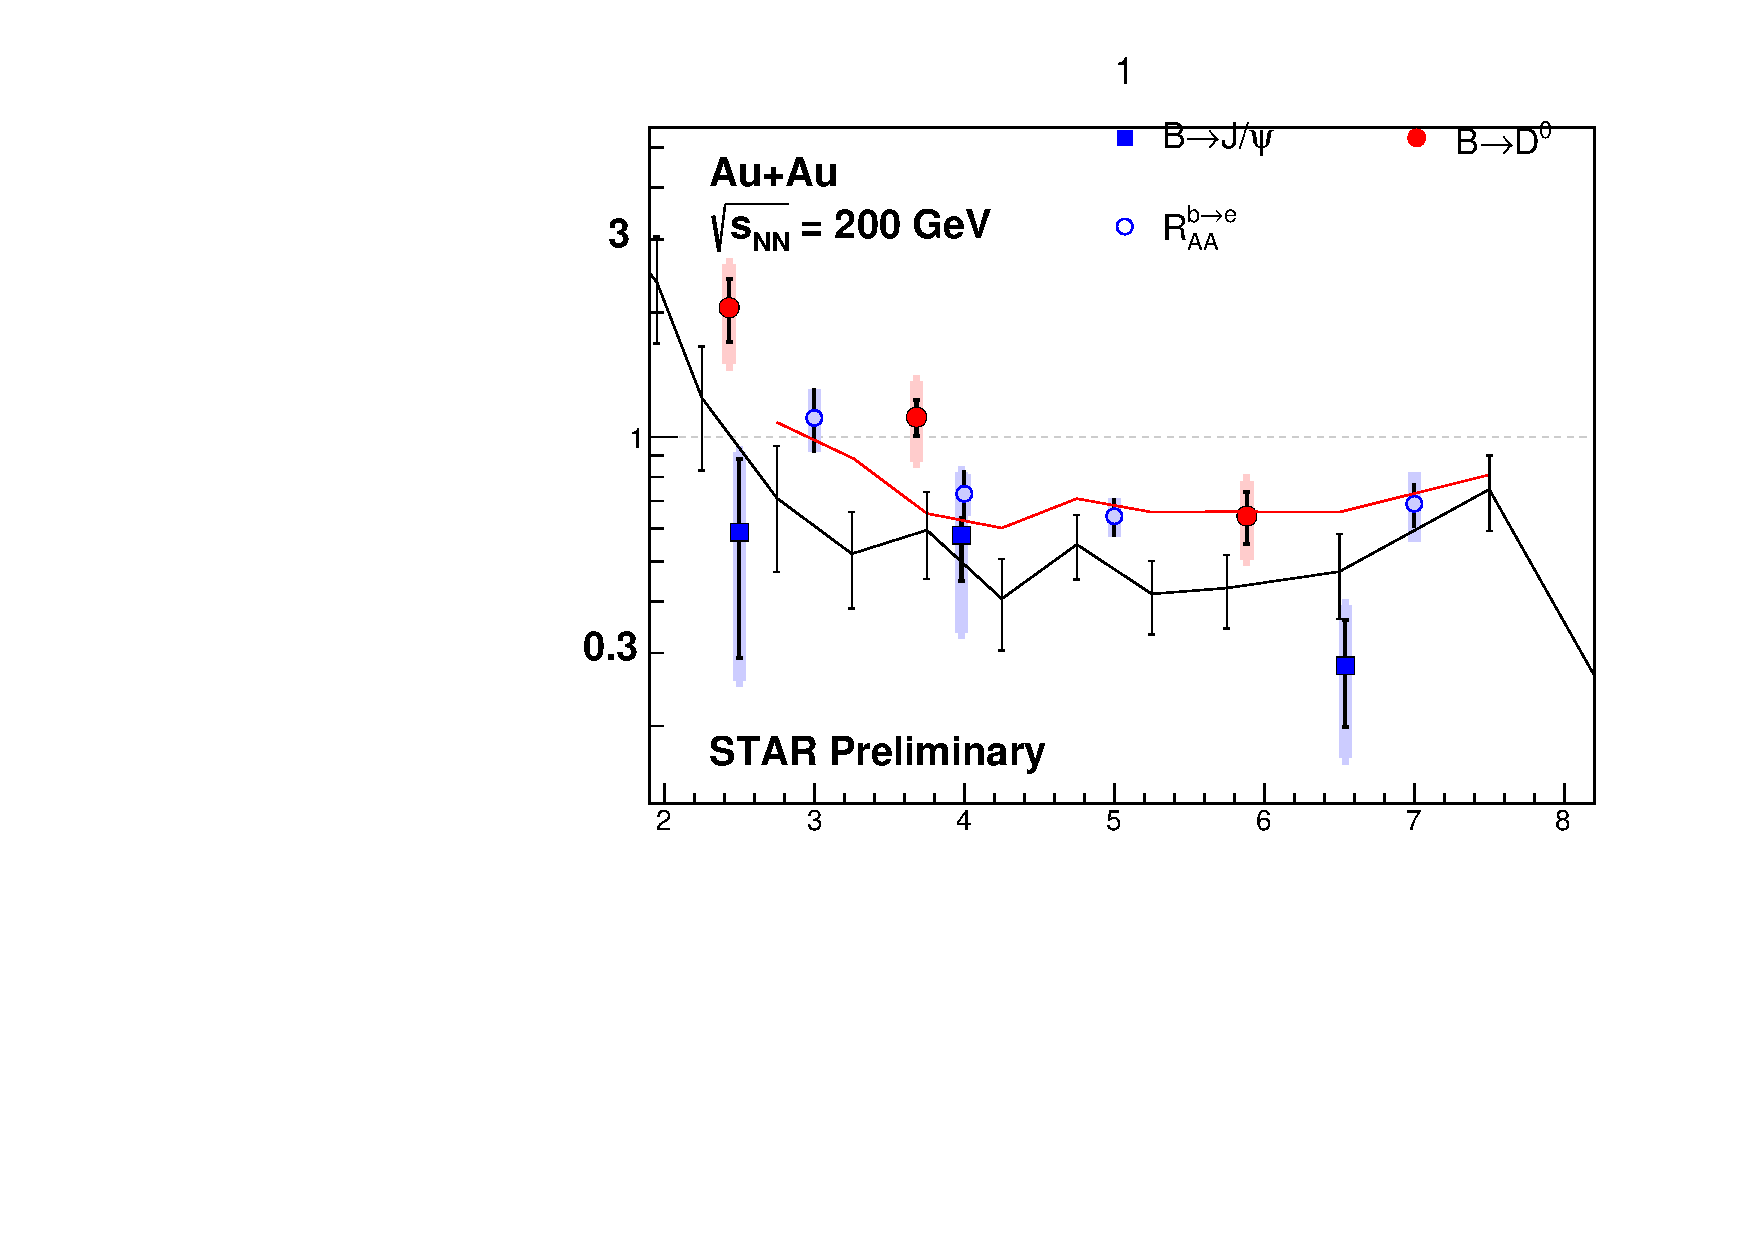
\includegraphics[width=8cm]{src/r.pdf}
	\caption{b$\to$e RAA数据不匹配的情况。黑线是用\cite{SI2020135465}Fig1除以\cite{Aidala:2019hib}得到的,红线是\cite{SI2020135465}Fig3的数据,背景数据点是\cite{Tang:2020ame}}
	\label{b2e}
\end{figure}
2. 由1说明,\cite{SI2020135465}分子pT的结论不准确,现在正在做的是用\ref{sec:拟合raa分母参数}的参数作为分母,用拟设的参数作为分子,算出Raa与实验\cite{Tang:2020ame}比较,接着用模拟退火法,求出分子最优的参数。仍然使用统计量$\displaystyle\chi=\frac{(o-e)^2}{e}$使它最小。现在做到的较好结果是$\chi^2=\num{1.524698}$. 使用默认参数(司凡提供的)的结果是$\chi^2=\num{2.197755}$. 其图像如图\ref{B1},\ref{B2}所示。
\begin{remark}
	背景的数据点以TCanvas形式存储在root文件中,现暂未找到调整坐标轴以及调整图表标题的方法。
\end{remark}

\begin{figure}[h]
\centering
\begin{minipage}[t]{0.48\textwidth}
\centering
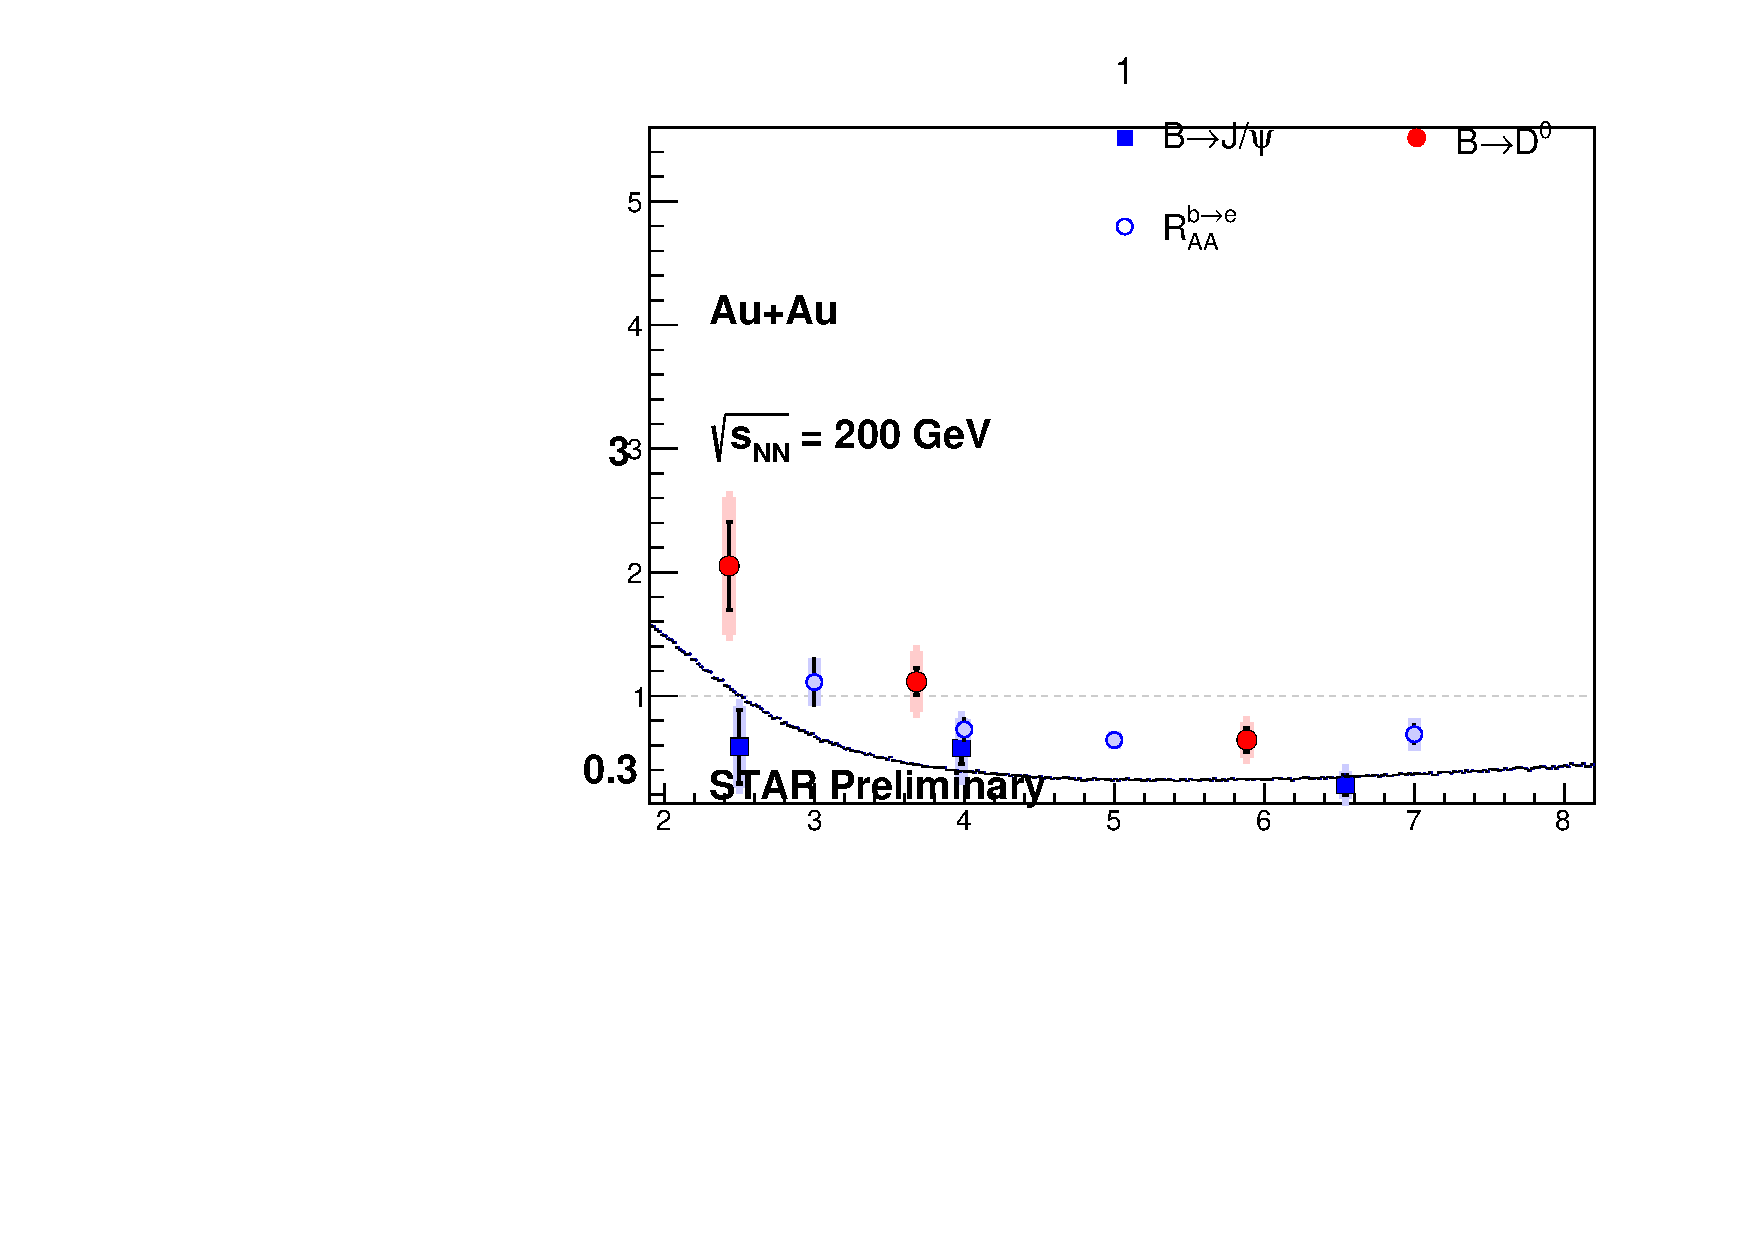
\includegraphics[width=6cm]{src/run1/graph/B2e.pdf}
\caption{B2e}
\end{minipage}
\begin{minipage}[t]{0.48\textwidth}
\centering
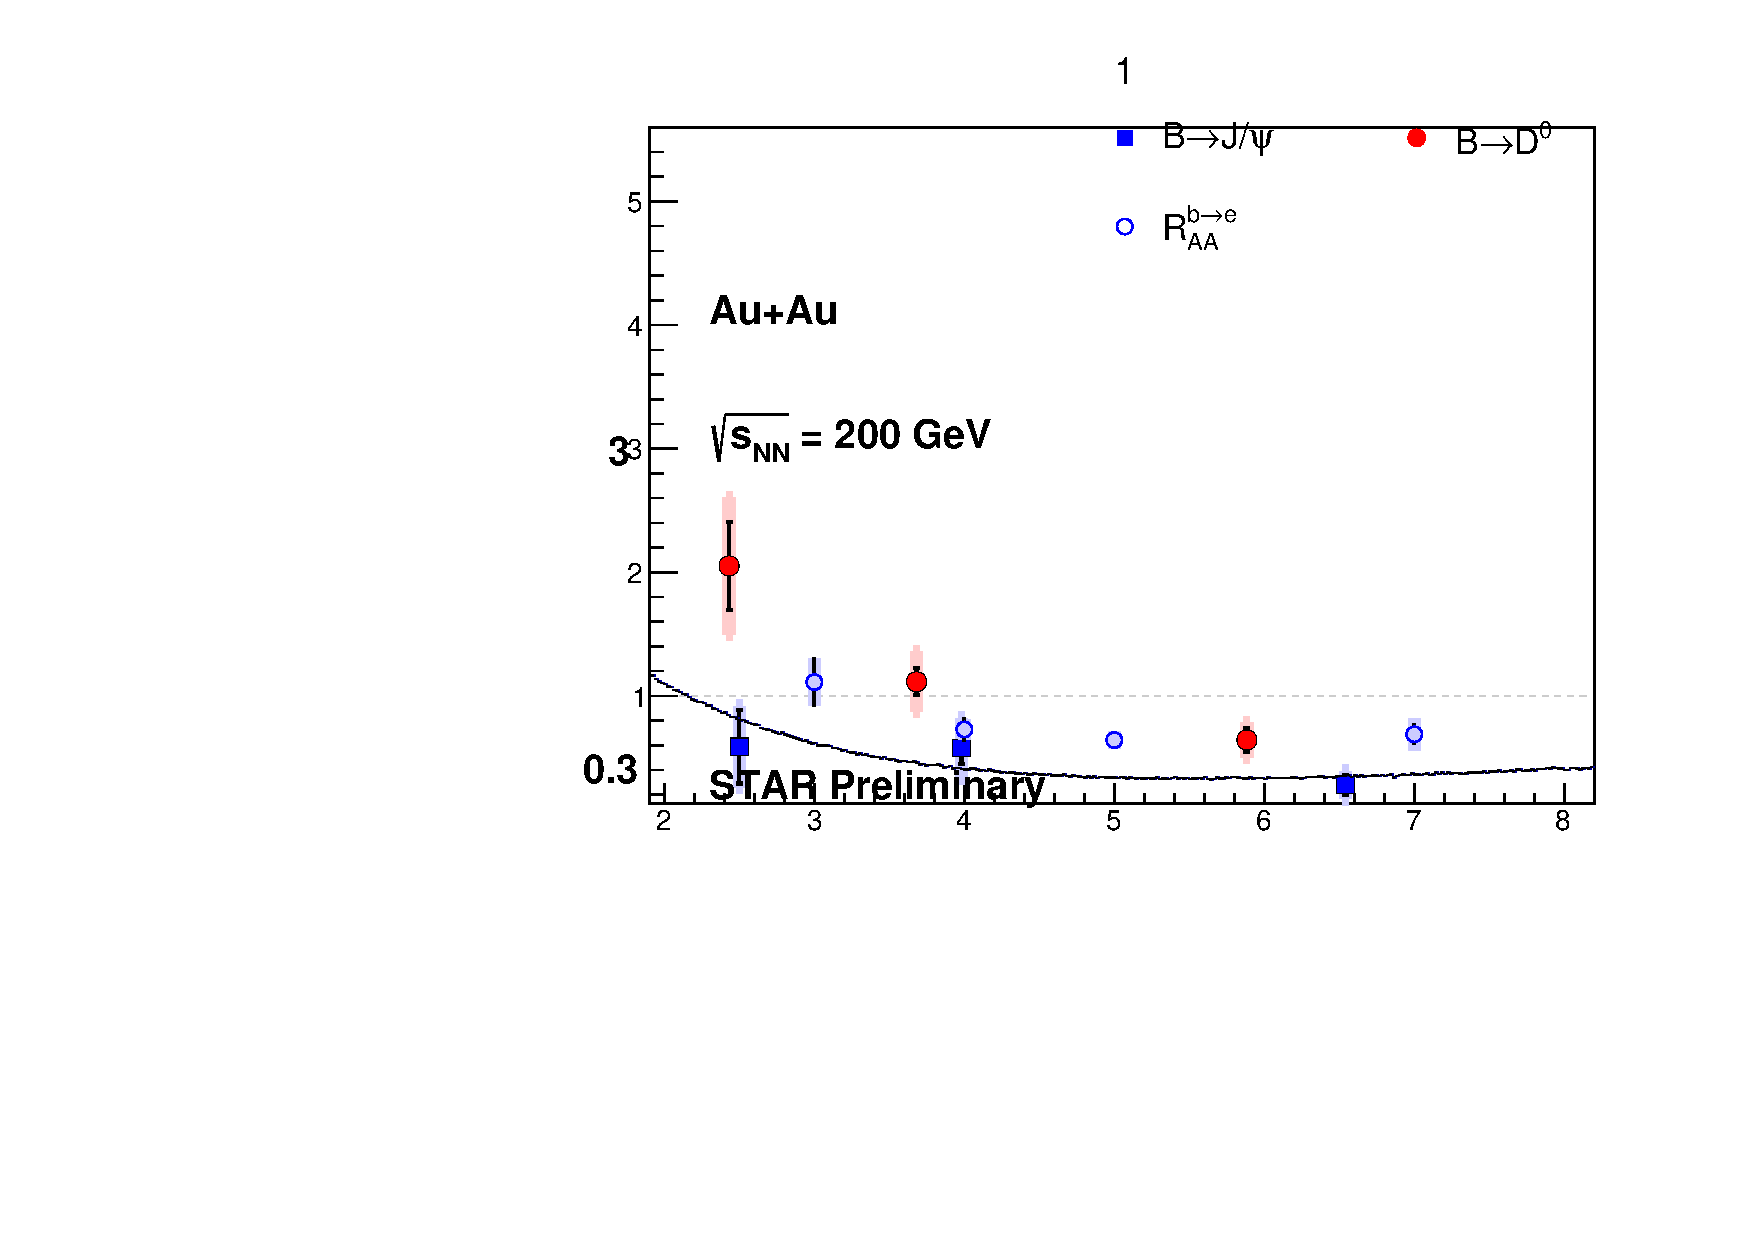
\includegraphics[width=6cm]{src/run1/graph/B2D0.pdf}
\caption{B2D0}
\end{minipage}
\begin{minipage}[t]{0.48\textwidth}
\centering
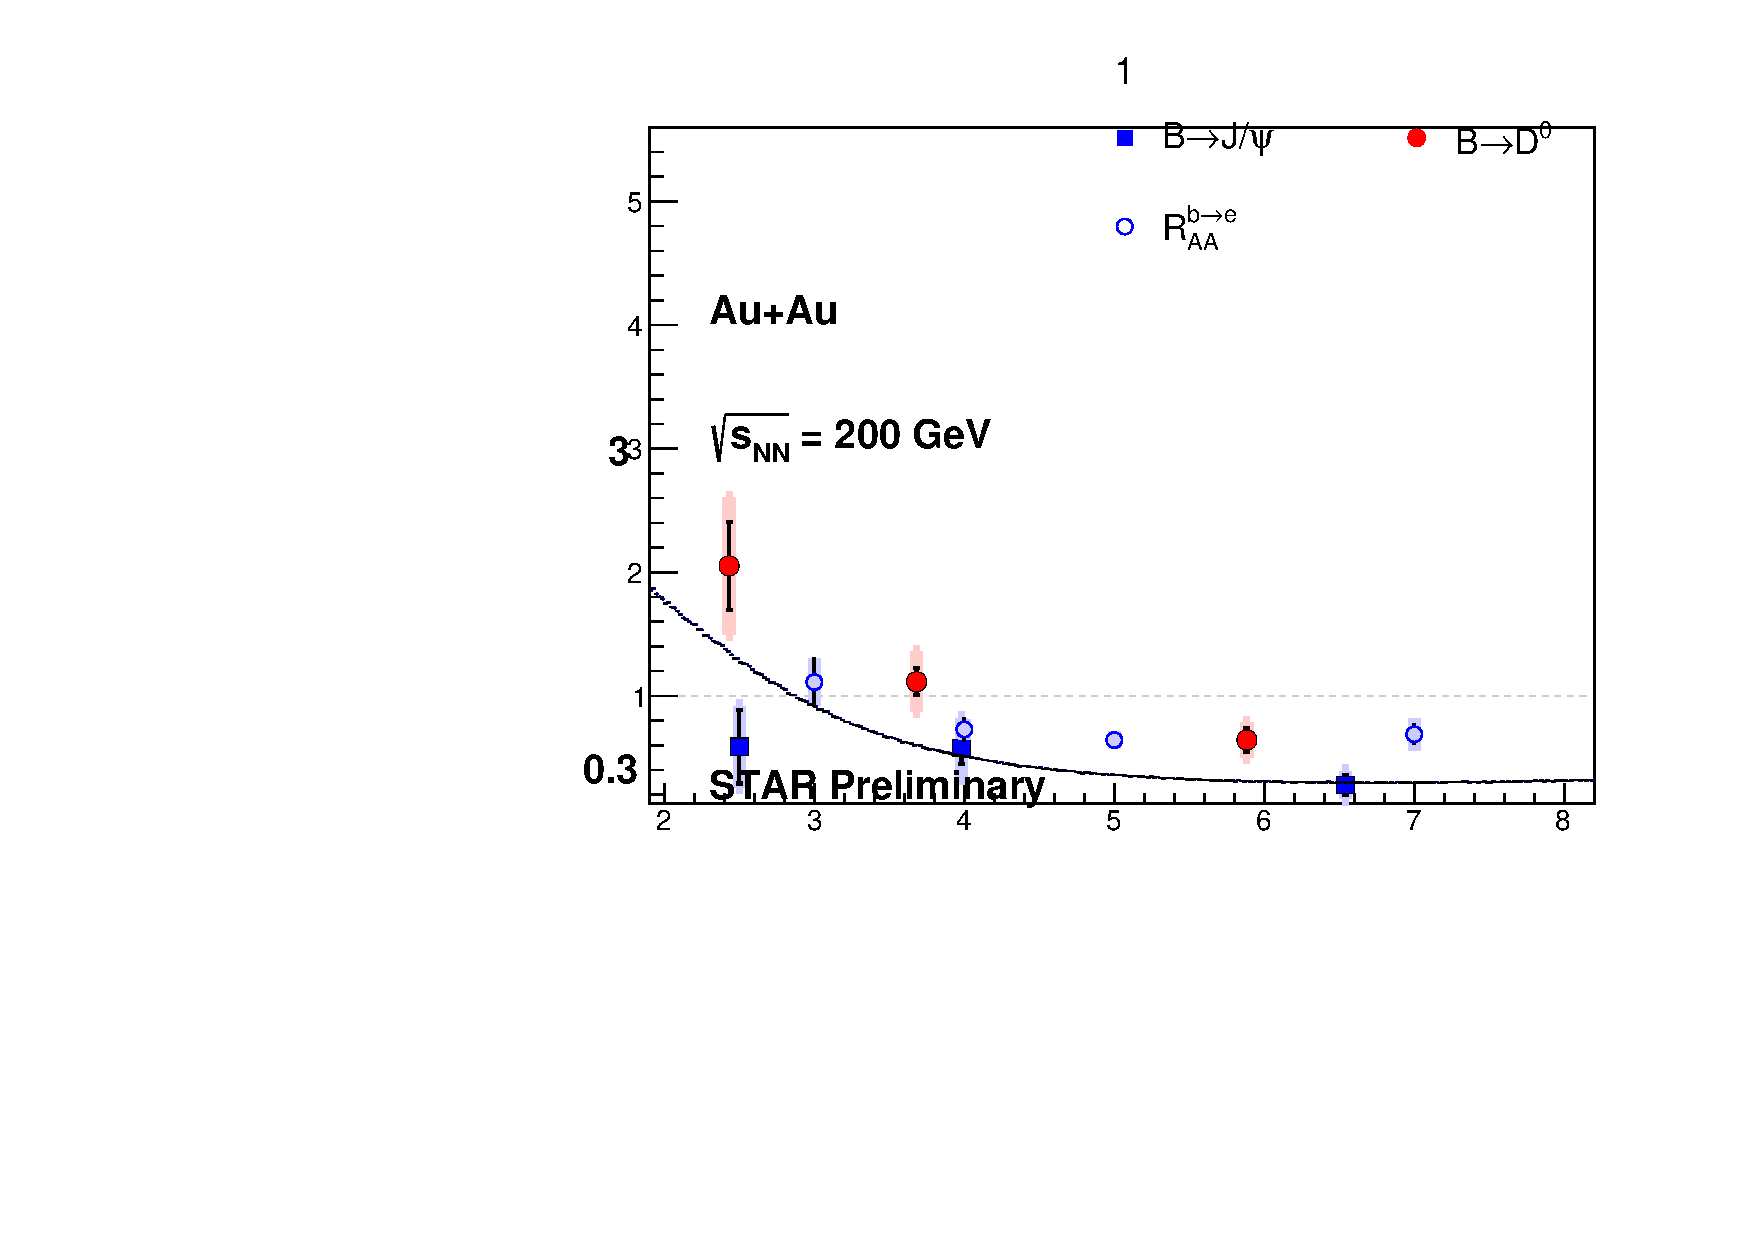
\includegraphics[width=6cm]{src/run1/graph/B2Jpsi.pdf}
\caption{B2Jpsi}
\end{minipage}
\label{B1}
\caption{默认参数,$\chi^2=\num{2.197755}$}
\end{figure}

\begin{figure}[h]
\centering
\begin{minipage}[t]{0.48\textwidth}
\centering
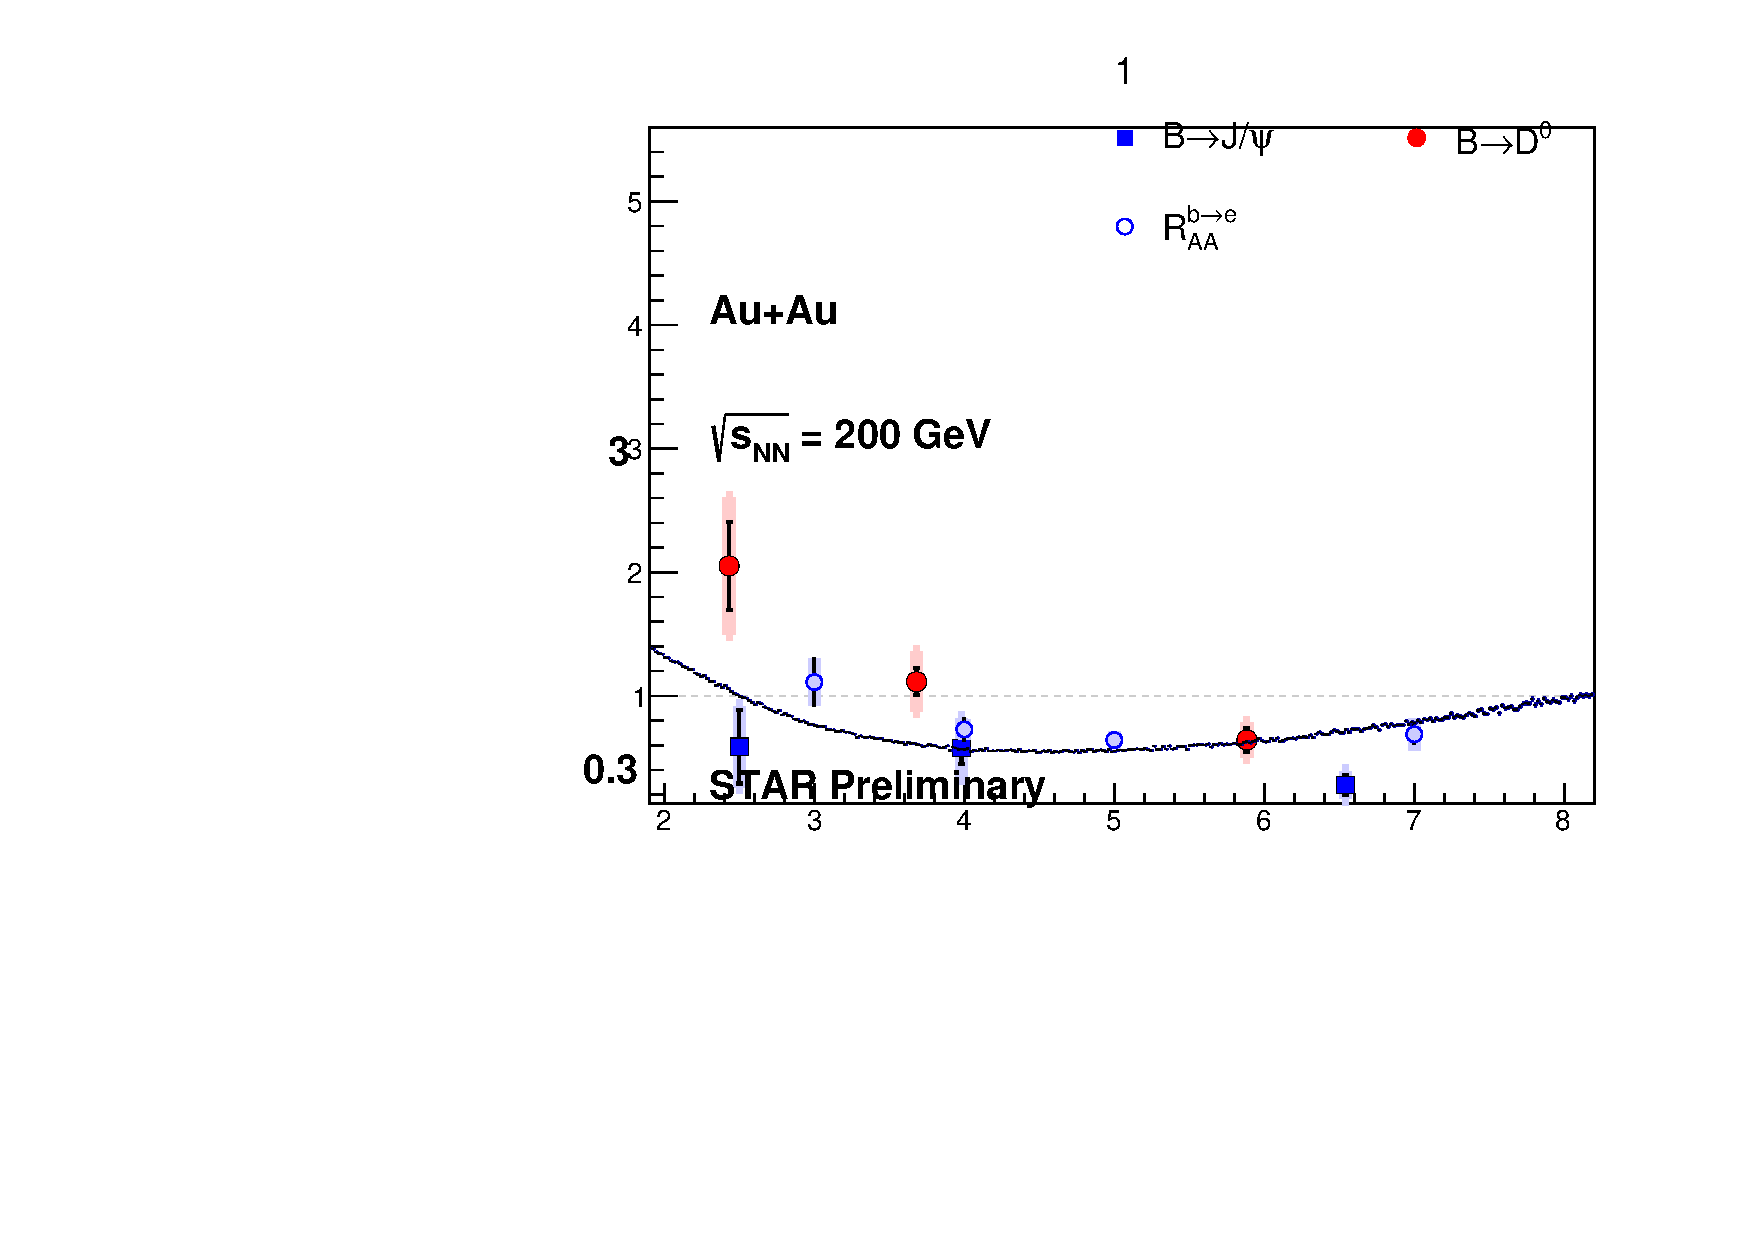
\includegraphics[width=6cm]{src/run125/graph/B2e.pdf}
\caption{B2e}
\end{minipage}
\begin{minipage}[t]{0.48\textwidth}
\centering
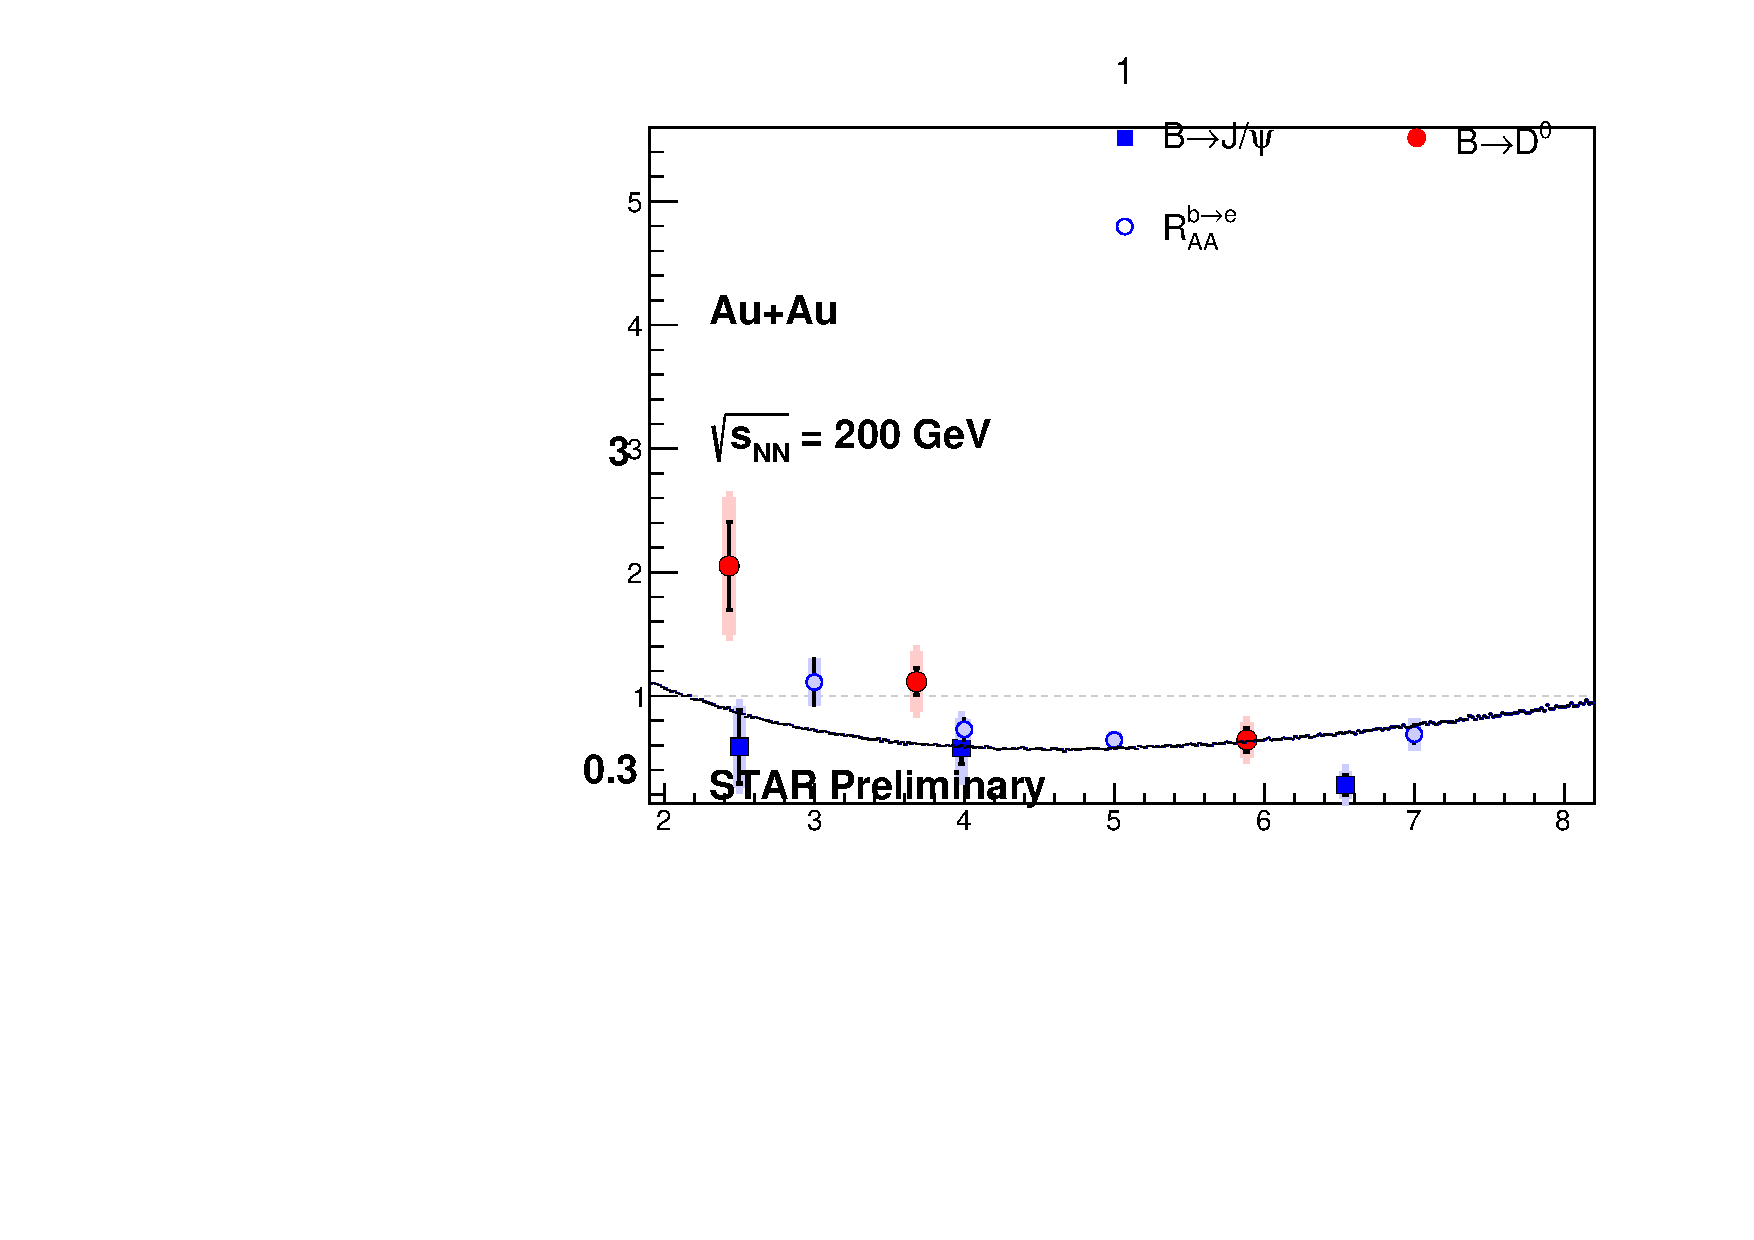
\includegraphics[width=6cm]{src/run125/graph/B2D0.pdf}
\caption{B2D0}
\end{minipage}
\begin{minipage}[t]{0.48\textwidth}
\centering
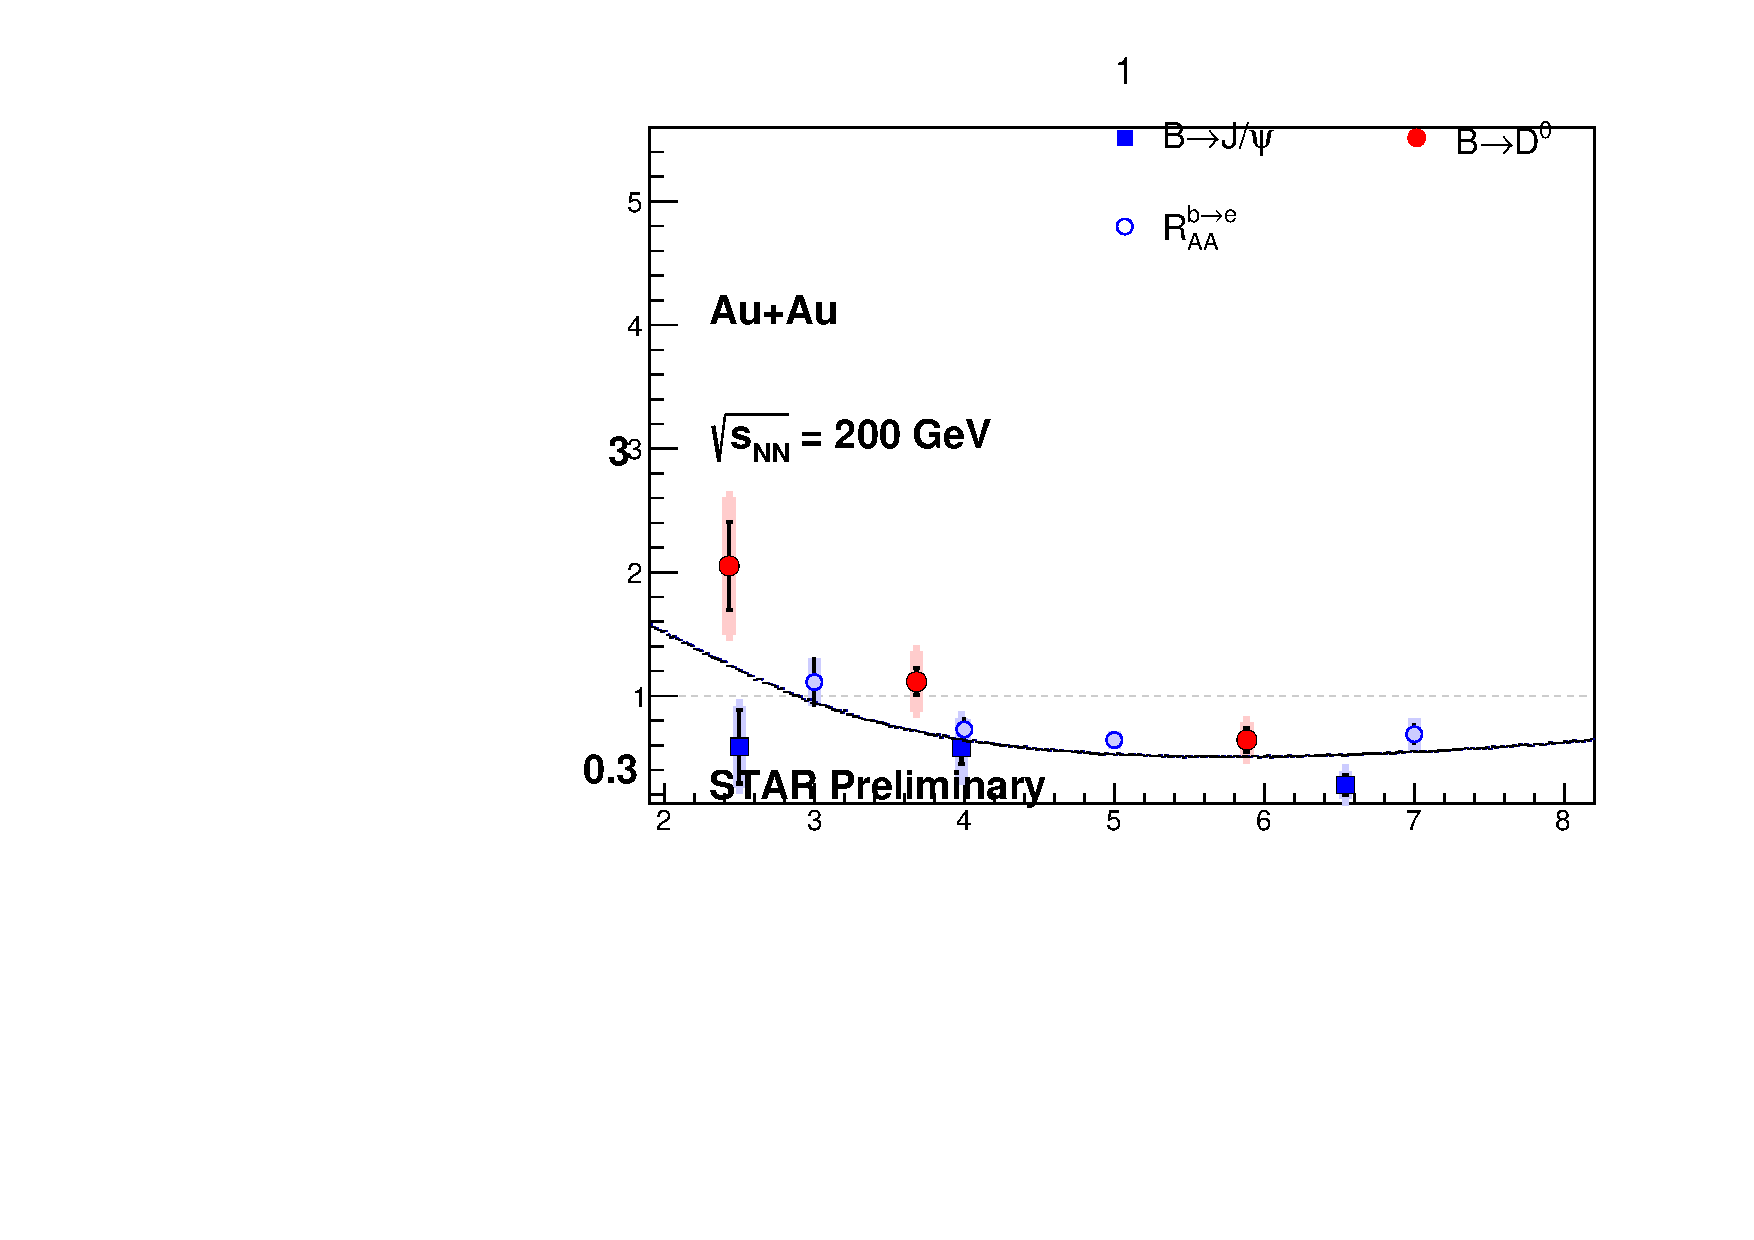
\includegraphics[width=6cm]{src/run125/graph/B2Jpsi.pdf}
\caption{B2Jpsi}
\end{minipage}
\label{B2}
\caption{默认参数,$\chi^2=\num{2.197755}$}
\end{figure}

% section 求raa (end)

\afterpage{\blankpage}
\bibliographystyle{unsrt}
\bibliography{report}
\end{document} 
